\exercise{Enhancement}
\subsection*{a - IPlogenhance}
Sometimes it can be desirable to increase the intensity of low-intensity pixels without enhancing high-intensity pixels too much. A way to achieve this goal is by compressing the dynamic range of an image. By applying the log transform an image may become more insightful than when the dynamic range is too large. The log transformation is: \[
                                                                                               s = c\mbox{ }log(1+r)
                                                                                              \]
In this formula the value $r$ represents the value of the pixel the transformation is applied to. The value $c$ is a constant chosen by the user. The following Matlab code applies the log transformation to an image. 
\matlabexternal{IPlogenhance.m}
Here the type of \verb image  is a $y \times x$-matrix. The output image is also an $y \times x$-matrix with the transformation applied.

\subsection*{b - Enhancing a fractured spine}
In order to make sure the implementation is correct and the log transformation is useful the operation is applied to an image that could benefit from a compressed dynamic range. Figures~\ref{fig:withoutEnhancement} and~\ref{fig:withEnhancement} are both pictures of a fractured spine, but figure~\ref{fig:withEnhancement} has the log transform applied to it with $c = 1.75$.
\begin{figure}
 \centering
 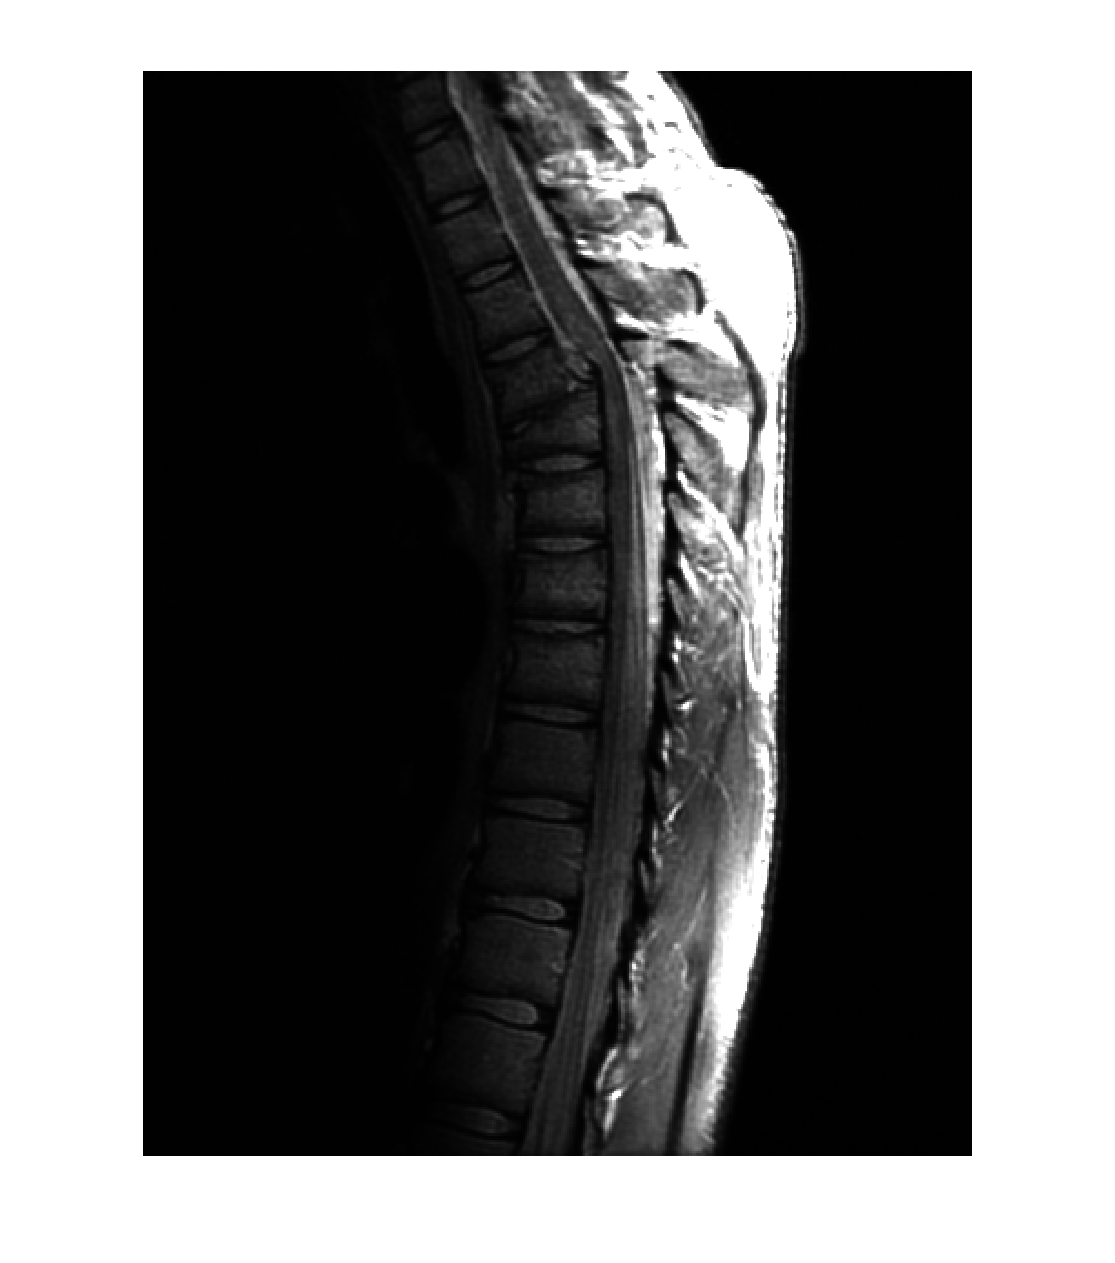
\includegraphics{breukLelijk.eps}
 \caption{An image of a fractured spine without enhancement applied}
 \label{fig:withoutEnhancement}
\end{figure}

\begin{figure}
 \centering
 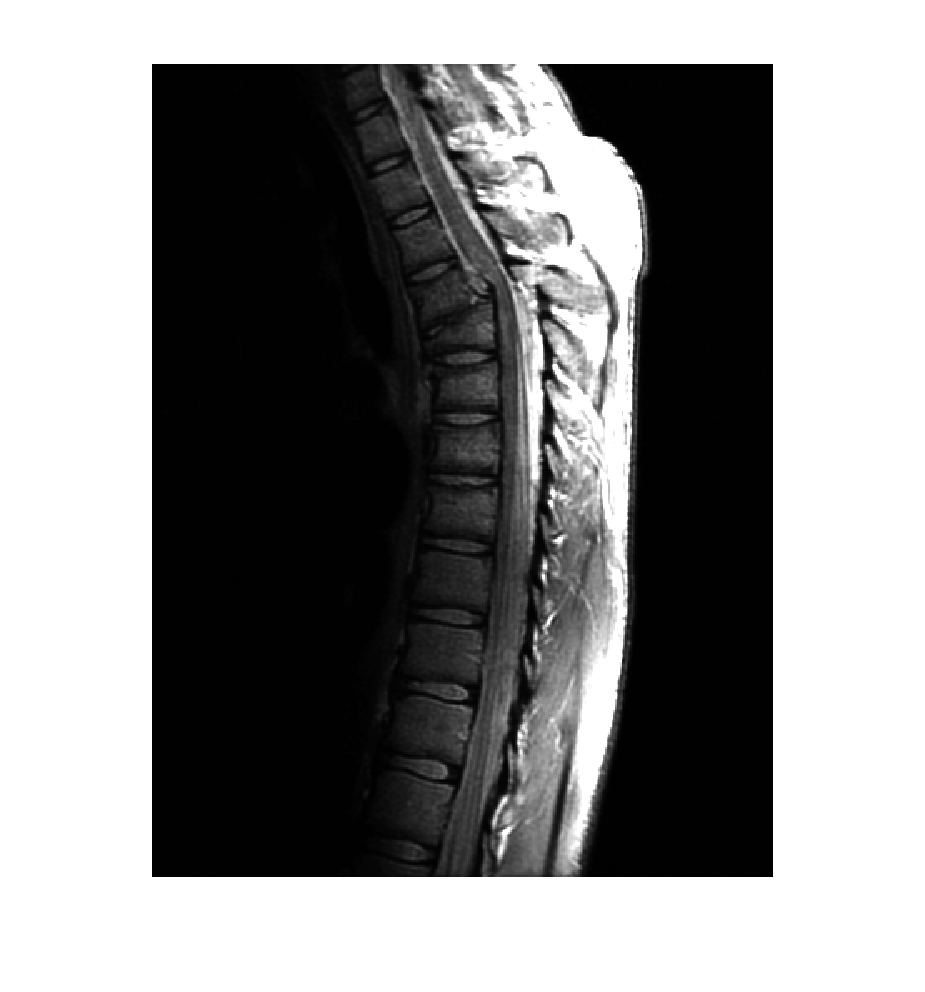
\includegraphics{breukMooi.eps}
 \caption{An image of a fractured spine with enhancement applied}
 \label{fig:withEnhancement}
\end{figure}
